\documentclass[tikz,border=4pt]{standalone}
\usepackage{amsmath}
\begin{document}
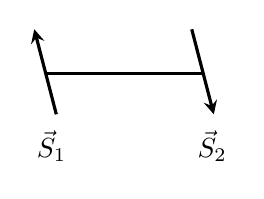
\begin{tikzpicture}[>=stealth, thick, scale=1.0]
  % Bond connecting two spins
  \draw[line width=0.9pt] (0, 0) -- (2.0, 0);

  % Spin S1 (up-left) and S2 (down-right)
  \draw[->, line width=1.15pt] (0.14, -0.52) -- (-0.14, 0.56);
  \draw[->, line width=1.15pt] (1.86, 0.56) -- (2.14, -0.52);

  \node[below] at (0.08, -0.60) {$\vec{S}_1$};
  \node[below] at (2.12, -0.60) {$\vec{S}_2$};
\end{tikzpicture}
\end{document}
